\documentclass[border=10pt]{standalone}
\usepackage{tikz}
\usepackage{amsmath}

\definecolor{inFill}{RGB}{183,224,177}
\definecolor{inLine}{RGB}{32,102,32}
\definecolor{hidFill}{RGB}{199,203,243}
\definecolor{hidLine}{RGB}{52,58,143}
\definecolor{outFill}{RGB}{243,199,199}
\definecolor{outLine}{RGB}{143,52,52}

\begin{document}
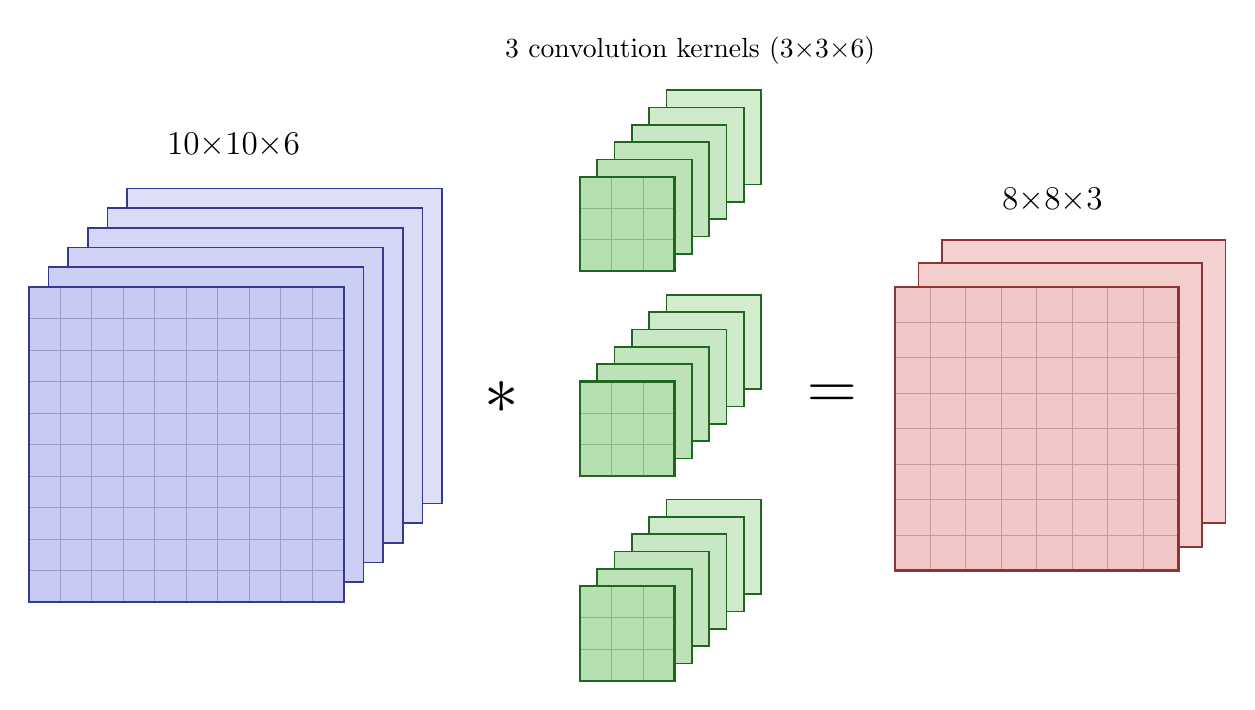
\begin{tikzpicture}[line width=0.8pt, font=\large]

  % ========== 特征图堆 10x10x6（淡紫）==========
  \newcommand{\fmstack}[2]{%
    \foreach \k in {5,4,...,0}{%
      \pgfmathtruncatemacro{\op}{100-8*\k}
      \fill[hidFill!\op, draw=hidLine, line width=0.6pt]
        ({#1+0.25*\k},{#2+0.25*\k}) rectangle ++(4,4);
    }
    \draw[hidLine!50, line width=0.25pt, shift={(#1,#2)}, step=0.4] (0,0) grid (4,4);
    \draw[hidLine] (#1,#2) rectangle ++(4,4);
  }

  % ========== 核堆 3x3x6（淡绿）==========
  \newcommand{\kstack}[2]{%
    \foreach \k in {5,4,...,0}{%
      \pgfmathtruncatemacro{\op}{100-8*\k}
      \fill[inFill!\op, draw=inLine, line width=0.6pt]
        ({#1+0.22*\k},{#2+0.22*\k}) rectangle ++(1.2,1.2);
    }
    \draw[inLine!50, line width=0.25pt, shift={(#1,#2)}, step=0.4] (0,0) grid (1.2,1.2);
    \draw[inLine] (#1,#2) rectangle ++(1.2,1.2);
  }

  % ========== 输出堆 8x8x3（淡红，与 input/核同款堆叠画法）==========
  \newcommand{\outstack}[2]{%
    \foreach \k in {2,1,0}{%
      \pgfmathtruncatemacro{\op}{100-10*\k}
      \fill[outFill!\op, draw=outLine, line width=0.6pt]
        ({#1+0.3*\k},{#2+0.3*\k}) rectangle ++(3.6,3.6);
    }
    \draw[outLine!50, line width=0.25pt, shift={(#1,#2)}, step=0.45] (0,0) grid (3.6,3.6);
    \draw[outLine] (#1,#2) rectangle ++(3.6,3.6);
  }

  % ================= 左：输入体积 =================
  \fmstack{0}{-2.2}
  \node at (2.6,3.6) {10$\times$10$\times$6};

  % ================= 中：运算符号（居中各一个）=================
  \node[font=\Huge] at (6.0,0.4)  {$\ast$};
  \node[font=\Huge] at (10.2,0.4) {$=$};

  % ================= 核列：3 个核竖排 =================
  \kstack{7.0}{2.0}
  \kstack{7.0}{-0.6}
  \kstack{7.0}{-3.2}
  % ★ 核列上方英文总标题
  \node[font=\normalsize] at (8.4,4.8) {3 convolution kernels (3$\times$3$\times$6)};

  % ================= 右：输出体积（★ 三层堆叠）=================
  \outstack{11.0}{-1.8}
  \node at (13.0,2.9) {8$\times$8$\times$3};

\end{tikzpicture}
\end{document}